	 	 	

\chapter{Registración de imágenes}

\section{Descripción general}
\label{sec:descripcion-general-registracion}

La registración de imágenes es el proceso de transformación de diferentes conjuntos de datos a un mismo sistema de coordenadas. Los imágenes a registrar pueden ser provistas por varios sensores, haber sido tomadas en diferentes épocas o desde distintos puntos de vista. Esta técnica se utiliza en diversas áreas, tales como visión por computador, tratamiento de imágenes médica, reconocimiento automático de objetivos, procesamiento de datos satelitales, entre otros. El producto de la registración permite comparar o integrar los datos obtenidos a partir de diferentes fuentes. \\
Una aplicación específica de la registración de imágenes, muy utilizada en el campo de la robótica, es la estimación de la odometría de un sensor en movimiento. En particular, la odometría visual determina los cambios en la posición y la orientación de la cámara entre pares de imágenes consecutivas en una secuencia de video. \\
En este trabajo, se sigue un enfoque de odometría visual para construir un mapa 3D de una superficie de interés, obtenido como resultado de un ensayo hidraulico en laboratorio, utilizando una cámara RGB-D Kinect. Como se describe en la sección \ref{cap:estado-del-arte}, el enfoque aplicado se inspira en un conjunto de trabajos anteriores, orientados al mapeo 3D de interiores, donde emplearon cámaras RGB-D. Varias de estas propuestas se basan en un proceso de reconstrucción acumulativo entre pares de frame RGB-D, conocido como \textit{Pairwise alignment} o \textit{alineación de pares}. Este método consiste en determinar la traslacion y rotacion del sensor, con seis grados de libertad, entre un frame de origen y otro de destino. \\
La solución \textit{Pairwise alignment} implementada en este trabajo se divide en las siguientes etapas:
\begin{enumerate}
\item Detección de características visuales 2D y cómputo de descriptores.

\item Emparejamiento de características visuales 2D.

\item Extracción de pares de puntos 3D asociado a las correspondencias de características 2D.

\item Eliminación de correspondencias erróneas (\textit{outliers}) entre puntos 3D.

\item Estimación de la transformación rígida, a partir de las correspondencias de puntos 3D filtradas en la etapa (4).

\item Refinamiento iterativo de la transformación utilizando el algoritmo ICP sobre el conjunto de puntos 3D obtenidos en la etapa (3), hasta cumplir un criterio de convergencia.
\end{enumerate}

En las siguientes secciones se describe con mayor detalle cada etapa del procedimiento de alineación de pares de \textit{frames}. Por ultimo, en la seccion \ref{sec:acumulacion-del-error-slam}, se expone el problema de la acumulacion de error que aparece al utilizar exclusivamente un enfoque de odometría y se motiva el uso de la técnica de optimización global, conocida como SLAM, que permite la construcción de mapas consistentes.

\section{Características visuales}
\label{sec:features}

La extracción de características (\textit{features}) visuales es una técnica muy utilizada en visión por computador para la detección, reconocimiento y seguimiento de objetos. Este procedimiento está compuesto por dos etapas : la detección de un punto de interés (\textit{keypoint}) que identifica un área relevante en la imagen, y el cómputo de un \textit{descriptor}, que caracteriza a la región. Por lo general, el algoritmo de detección identifica regiones con gran variación de intensidad, por ejemplo bordes o esquinas de un objeto, y se selecciona el centro de la región como \textit{keypoint}. El \textit{descriptor} se representa como un vector multidimensional, que suele calcularse en función de ciertas métricas (por ejemplo la orientación o la escala) utilizando los puntos circundantes al \textit{keypoint}. Dependiendo el tipo de aplicación puede desearse que las características sean invariantes a diferentes transformaciones, entre ellas, rotación, traslación, cambios de iluminación y escala. En las siguientes secciones se presentan los algoritmos SURF y ORB, considerados actualmente parte del estado del arte en la detección y descripción de características visuales.

\subsection{Speeded Up Robust Feature (SURF)}

SURF\cite{bay2008speeded} es un detector y descriptor de características visuales inspirado por el descriptor de SIFT\cite{Lowe04}. Su principal diferencia radica en su velocidad, siendo la versión estándar de SURF un orden magnitud más rápido que SIFT, y según sus autores, más robusto ante diferentes tipos de transformaciones.

\subsubsection{El detector de caracterısticas de SURF}
EL detector de SURF se basa en el determinante de la matriz Hessiana. Dada una función continua $ f(x, y) $, la matriz Hessiana \textit{H} está formada por las derivadas parciales de \textit{f}:

\begin{equation}
H(f(x, y)) =
\left(
\begin{array}{cc}
\frac{\partial^2 f}{\partial x^2} & \frac{\partial^2 f}{{\partial x}{\partial y}} \\
\frac{\partial^2 f}{{\partial x}{\partial y}} & \frac{\partial^2 f}{\partial y^2} \\
\end{array}
\right)
\end{equation}

Siendo el determinante de esta matriz :

\begin{equation}
det(H) = \frac{\partial^2 f}{\partial x^2} \frac{\partial^2 f}{\partial y^2}
	 - \left( \frac{\partial^2 f}{{\partial x}{\partial y}} \right)^ 2
\end{equation}

A partir del test de la segunda derivada
\footnote{Si la Hessiana es definida positiva en \textbf{x}, entonces \textit{f(\textbf{x})} tiene un mínimo local en \textbf{x}. Si la Hessiana es definida negativa, entonces \textit{f(\textbf{x})} tiene un máximo local en \textbf{x}. Si la Hessiana tiene autovalores positivos y negativos, \textit{f(\textbf{x})} es un punto de silla. En otro caso el test no aporta información.}
se tiene que si el determinante es positivo se puede clasificar a ese punto de la función como un máximo o mínimo local, mientras que si es negativo se concluye que no es un extremo local.

Al aplicar esta teoría al dominio de las imágenes, se sustituye $f(x,y)$ por la intensidad de los pixeles de la imagen $I(x,y)$ y se reemplaza el cálculo de las derivadas parciales por la aplicación de filtros de convolución. En particular, para calcular las derivadas parciales se pueden utilizar filtros de convolución que discretizan las derivadas parciales segundas de la función Gaussiana. Sin embargo, los autores de SURF proponen una aproximación a estos filtros por medio de \textit{box filters}. Como se observa en la figura \ref{fig:box-filters}, los \textit{box filters} son filtros de convolución muy simples, que pueden ser implementados eficientemente utilizando la representación de la \textit{imagen integral}\cite{wiki-imagen-integral}.

\begin{figure}[ht]
\centering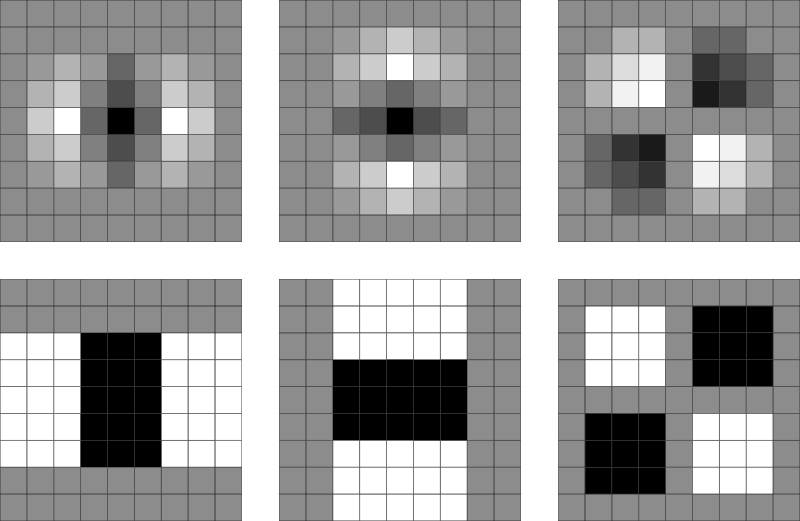
\includegraphics[width=\imsize]
{box-filters}
\caption[Box filters]
{Arriba: Versión discreta de los filtros de las derivadas parciales segundas de la función Gaussiana con respecto a \textit{x}, \textit{y} y \textit{xy} respectivamente, denominadas $L_{xx}$, $L_{yy}$ y $L_{xy}$. Abajo: aproximaciones a los filtros de arriba mediante \textit{box filters} denotados $D_{xx}$, $D_{yy}$ y $D_{xy}$ respectivamente. Imagen original: \cite{bay2008speeded}.}
\label{fig:box-filters}
\end{figure}

Para calcular el determinante de la Hessiana por medio de \textit{box filters} se utiliza una aproximación, denominada \textit{blob response} en la posición $(x, y, \sigma)$, que se define como :
\begin{equation}
det(H_{approx}) = D_{xx}D_{yy} - (0.9D_{xy})^2
\end{equation}

Para encontrar las características visuales se utiliza el concepto de espacio de escalas\cite{wiki-scale-space}(\textit{scale space}). El espacio de escalas de una imagen \textit{I} es una función continua, parametrizada en \textit{t}, que representa un conjunto (infinito) de imágenes, obtenidas a partir de suavizar \textit{I}, donde \textit{t} define el grado de suavizamiento. Tradicionalmente, un \textit{scale space} se suele implementar como una pirámide imágenes donde iterativamente se aplican filtros de suavizado por convolución y se reduce el tamaño de la imagen. Este método se aplica en SIFT, pero es computacionalmente costoso debido al re-escalado de las imágenes. En SURF, se implementa un enfoque diferente, basado en que la convolución con \textit{box filters} utilizando la representación de la imagen integral no depende del tamaño del filtro, por lo que, conceptualmente se construye una pirámide de filtros para aplicar sobre la imagen original. De esta forma, se puede calcular el \textit{blob response} en varias escalas en paralelo, sin necesidad de re-escalar la imagen. En la figura \ref{fig:scale-space} se ilustra la diferencia entre el enfoque aplicado en SIFT y el propuesto en SURF para la construcción del espacio de escalas.

\begin{figure}[ht]
\centering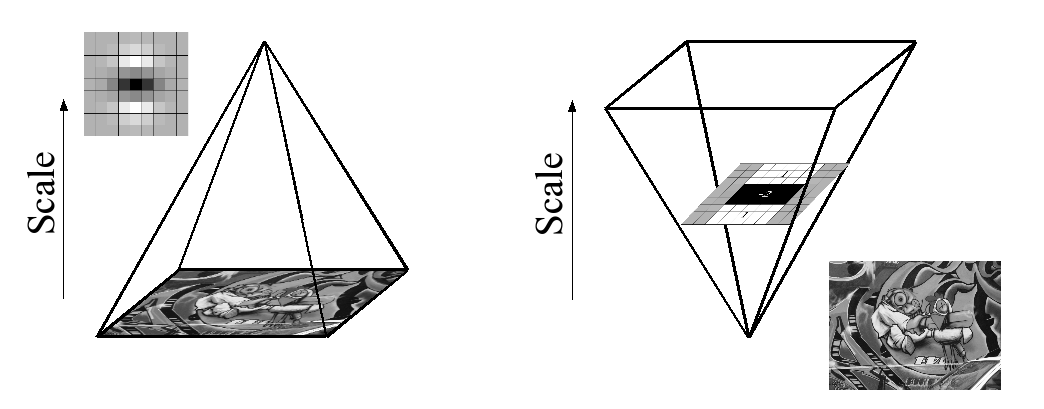
\includegraphics[width=\imsizeL]
{scale-space}
\caption[Espacio de escalas]
{Enfoques para construir el espacio de escalas. Izquierda: enfoque tradicional donde iterativamente se reescala la imagen y se suaviza con un filtro Gaussiano de un determinado tamaño. Derecha: enfoque propuesto por SURF donde aplican filtros de diferente tamaño (utilizando la imagen integral) manteniendo la imagen original. Fuente: \cite{bay2008speeded}.}
\label{fig:scale-space}
\end{figure}

El proceso de detección SURF se divide en 3 etapas:
\begin{itemize}
\item Filtrado de \textit{blob responses}: se eliminan características con respuesta por debajo de un umbral. Al incrementar el umbral se reduce la cantidad de características detectadas dejando la más robustas.

\item Aplicación del algoritmo de \textit{non-maximal suppresion}: se compara el píxel candidato con sus 26 vecinos (8 en la escala del candidato y 9 en las escalas superior e inferior) y se descarta si su respuesta no es máxima.

\item Interpolación: se interpolan los datos en la cercanía del candidato para obtener una localización con precisión de subpixel.

\end{itemize}

\subsubsection{El descriptor de SURF}
El descriptor de SURF describe cómo se distribuye la intensidad de los píxeles circundantes al centro de la característica. El cómputo del descriptor tiene 2 etapas: la extracción de la orientación
\footnote{Para algunas aplicaciones, la invarianza de rotación no es necesaria, por lo que se puede evitar el cálculo de la orientación, dando lugar al denominado Upright SURF (U-SURF).}
predominante de la característica y el cómputo de los componentes del vector utilizando \textit{Haar wavelets}. Los \textit{Haars wavelets} son filtros de convolución que se utilizan para calcular los gradientes de intensidad en \textit{x} y \textit{y}. Como se observa en la figura \ref{fig:haar-wavelet}, la convolución con \textit{Haar wavelets} puede ser implementada de forma eficiente, utilizando la representación de la imagen integral.

\begin{figure}[ht]
\centering
\begin{minipage}[h]{.45\textwidth}
\begin{center}
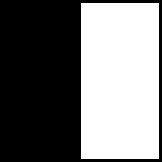
\includegraphics[width=0.5\textwidth]{haar-wavelet-x}
\end{center}
\end{minipage}
\hfill
\begin{minipage}[h]{.45\textwidth}
\begin{center}
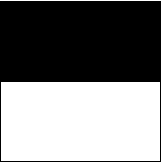
\includegraphics[width=0.5\textwidth]{haar-wavelet-y}
\end{center}
\end{minipage}
\hfill
\caption[Haar wavelet]{Filtros \textit{Haar wavelet} utilizados para computar los gradientes en la dirección \textit{x} (izquierda) e \textit{y} (derecha). La zona negra representa el valor −1, mientras que la blanca +1. Imagen original: \cite{bay2008speeded}.}
\label{fig:haar-wavelet}
\end{figure}

Para extraer la orientación de una \textit{feature} se deben realizar 2 tareas:
\begin{enumerate}

\item Computar las respuestas \textit{Haar wavelet} de tamaño $4\sigma$ (escala asociada al punto de interés) en un radio de $6\sigma$ alrededor del \textit{keypoint}, para obtener las componentes \textit{x, y} del gradiente de intensidades. A las respuestas obtenidas, se les aplica una Gaussiana (con desviación estándar de $2\sigma$) centrada en el punto de interés. Para cada píxel del área circular, se les asocia un punto 2D en el espacio dado por el vector gradiente.

\item Selección de la dirección predominante de las respuestas. Se rota una ventana de tamaño $\pi/3$ alrededor del keypoint y se suman las componentes de las respuestas dentro de la sección. El vector resultante con mayor módulo representa la orientación predominante del punto de interés. El procedimiento se ilustra en la figura \ref{fig:orientacion-surf}.

\end{enumerate}

\begin{figure}[ht]
\centering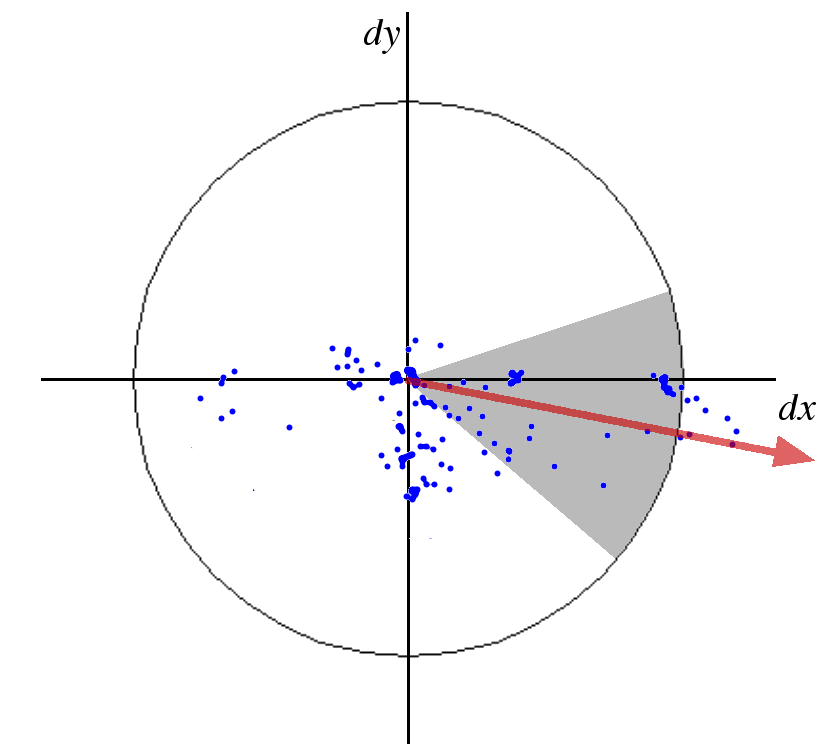
\includegraphics[width=\imsize]
{orientacion-surf}
\caption[Cálculo de la orientación para una característica SURF]
{La orientación dominante de la característica se encuentra rotando una ventana de tamaño $pi/3$ alrededor del keypoint, sumando las componentes de las respuestas producidas por los filtros \textit{Haar wavelets} dentro de la ventana y seleccionando la orientación del vector resultante con mayor módulo. Fuente: \cite{bay2008speeded}.}
\label{fig:orientacion-surf}
\end{figure}

Para extraer los componentes del descriptor, el primer paso consiste en construir una región rectangular de tamaño $20\sigma$ alrededor de la característica y orientada en la dirección predominante obtenida en la etapa anterior. La región se divide en $4 \times 4$ subregiones rectangulares, y para cada una se computa la respuesta de \textit{Haar wavelet} de tamaño $2\sigma$ sobre 25 puntos distribuidos regularmente. Denotando \textit{dx, dy} a las respuestas en la dirección \textit{x, y} respectivamente, se obtiene para cada subregión un vector de la forma:
\begin{equation}
\textbf{v} = \left[\sum{dx}, \sum{dy}, \sum{\abs{dx}}, \sum{\abs{dy}}\right]
\end{equation}
El descriptor resultante se compone por los vectores de cada subregión, por lo tiene un tamaño de $ 4 \times 4 \times 4 = 64 $ elementos.

\begin{figure}[ht]
\centering
\begin{minipage}[h]{.45\textwidth}
\begin{center}
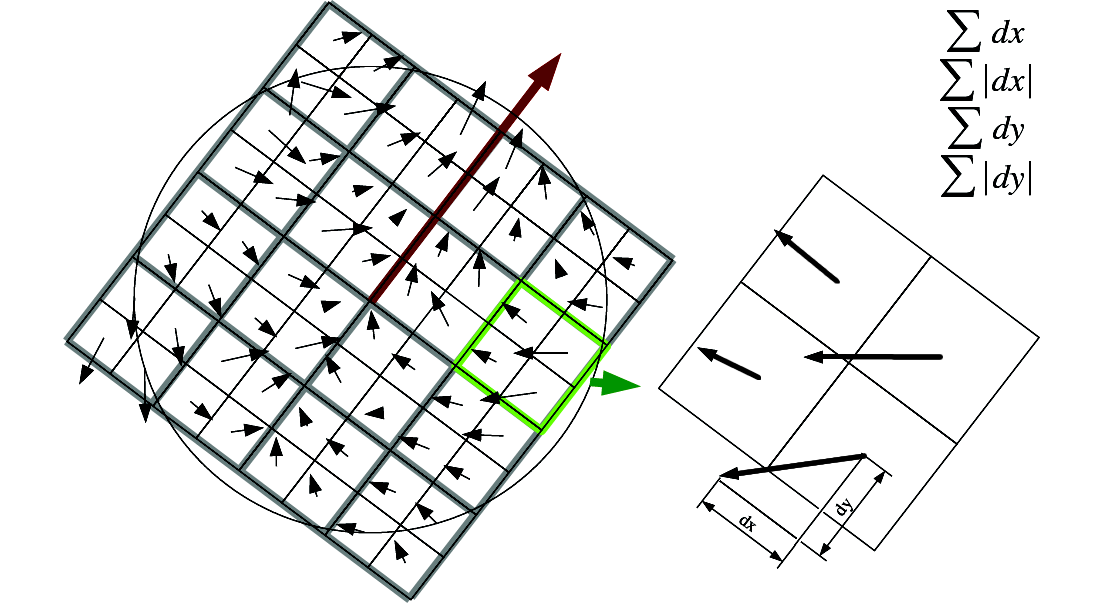
\includegraphics[width=\imsizeS]{grilla-surf}
\end{center}
\end{minipage}
\hfill
\begin{minipage}[h]{.45\textwidth}
\begin{center}
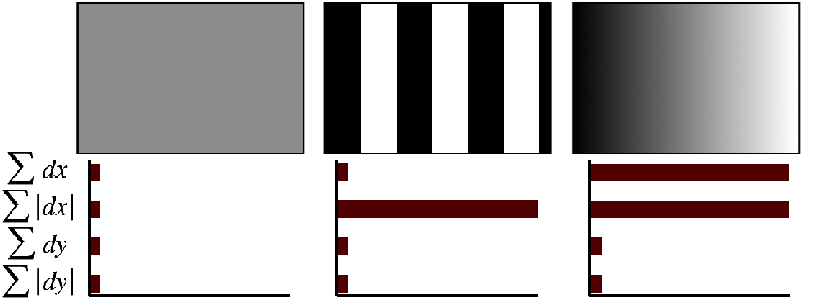
\includegraphics[width=\imsizeS]{histogramas-surf}
\end{center}
\end{minipage}
\hfill
\caption[Componentes del descriptor SURF]
{Izquierda: Cálculo de las componentes del descriptor. El rectángulo marcado limita una de las 16 sub-regiones, en las que se calcula la respuesta a los \textit{Haar wavelets} relativas a la orientación predominante de la característica. Derecha: componentes del descriptor SURF calculados para tres subregiones diferentes. Imagen original: \cite{bay2008speeded}.}
\label{fig:componentes-descriptor-surf}
\end{figure}

\subsection{Oriented FAST and Rotated BRIEF (ORB)}

ORB\cite{RubleeRKB11} es un detector y descriptor de características basado en el detector FAST\cite{Rosten06machinelearning} y el descriptor BRIEF\cite{Calonder12}. Si bien BRIEF es robusto ante cambios de iluminación y presencia de ruido, es muy sensible a rotaciones en el plano(\textit{in-plane}). Teniendo en cuenta este problema, ORB extiende FAST para detectar la orientación de las características (tipo \textit{corner}) y aplica mejoras sobre BRIEF dirigidas a aprovechar la información de orientación.

\subsubsection{Oriented FAST (oFAST)}

La detección de características oFAST se compone de 4 etapas :
\begin{enumerate}

\item Detección de características FAST. Se utiliza un umbral \textsl{t} de intensidad apropiado entre el píxel del centro y los pixeles del anillo circular. En oFAST se utiliza FAST-9 (radio del anillo de 9 pixeles) porque se comprobó que ofrece buenos resultados.

\item FAST no produce una medida de la bondad de los \textit{corners} y responde positivamente ante la presencia de bordes, por lo que en oFAST se realiza un filtrado con el fin de detectar las mejores características. Para obtener los mejores N \textit{corners}, se aplica una medida de bondad de los \textit{corners} dada por Harris\cite{Harris88alvey}, se ordenan las características en función de esa medida y se seleccionan las N mejores. Se establece un umbral suficientemente bajo para la bondad de los \textit{corners}, de forma tal de obtener al menos N características.

\item FAST no produce características multi-escala. Para solventar este problema, se construye una pirámide de escalas de la imagen (similar a SIFT y SURF), se calcula FAST (filtrado por Harris) en cada nivel y se aplica interpolación para obtener mejores resultados.

\item Estimación de la orientación. Para calcular la orientación se utiliza una medida muy simple conocida como \textit{centroide de intensidad (intensity centroid)}. Rosin\cite{Rosin99measuringcorner} define los momentos de un patch (área rectangular) de la siguiente forma:
\begin{equation}
m_{pq} = \sum_{x,y} x^{p}y^{q}I(x,y)
\end{equation}
Con estos momentos, se obtiene el \textit{intensity centroid} del patch de la siguiente forma:
\begin{equation}
C = \left(
\frac{m_{10}}{m_{00}} , \frac{m_{01}}{m_{00}} \\
\right)
\end{equation}
Se puede construir un vector $\vec{OC}$ desde el centro del corner O hacia el \textit{intensity centroid} C, y calcular la orientación del \textit{patch} centrado en la característica como:
\begin{equation}
\theta = atan2(m_{01}, m_{10})
\end{equation}

\end{enumerate}

\subsubsection{Rotated BRIEF (rBRIEF)}

\paragraph{Binary Robust Independent Elementary Features (BRIEF)}

Dado que el descriptor de ORB es una modificación de BRIEF, se presenta este último brevemente. El descriptor BRIEF\cite{Calonder12} es una cadena de bits (\textit{bit string}) que describe un \textit{patch} (centrado en el \textit{\textsl{keypoint}}) de la imagen. Está formado por un conjunto de tests binarios aplicados sobre los pixeles. Dado un \textit{patch} \textbf{p} de la imagen suavizada (para obtener mayor robustez frente al ruido), un test binario se define como:

\begin{equation}
\tau(\textbf{p}; \textbf{x}, \textbf{y}) := \left\lbrace
\begin{array}{cc}
1 & \textbf{p}(\textbf{x}) < \textbf{p}(\textbf{y}) \\
0 & \textbf{p}(\textbf{x}) >= \textbf{p}(\textbf{y}) \\
\end{array}
\right.
\end{equation}

donde \textbf{p}(\textbf{x}) es el valor de intensidad de \textbf{p} en la posición \textbf{x}.
El descriptor se define como un vector de n tests binarios :
\begin{equation}
f_{n}(\textbf{p}) := \sum_{i=1}^{n} 2^{i-1}\tau(\textbf{p}; \textbf{x}_{i}, \textbf{y}_{i})
\end{equation}

Hay varios enfoques para seleccionar el conjunto de posiciones a testear. En la versión estándar de BRIEF, se aplica una distribución Gaussiana alrededor del centro del \textit{patch} debido a que se comprobó muy buenos resultados.

\paragraph{Mejoras aplicadas en rBRIEF}

BRIEF posee 2 características importantes para un descriptor :
\begin{itemize}

\item Descriptores con elevada varianza y una media cercana a 0.5, lo que permite diferenciar descriptores más fácilmente, dado que distintas características responden de forma diferente.

\item Tests poco correlacionados, para que cada uno de ellos aporte información distinta y disminuya la redundancia.

\end{itemize}

Estas cualidades se ven disminuidas al agregar la información de orientación. Para solventar este problema, se sigue un enfoque de aprendizaje, por medio del cual se determinan un conjunto de pares de píxeles para ser comparados en cada test. \\
Para comenzar se obtienen los \textit{patches} centrados en cada keypoint oFAST extraídos a partir de un conjunto de imágenes de entrenamiento. Cada test es un par de sub-ventanas $5 \times 5$ píxeles de un \textit{patch} de $31 \times 31$. De todos los posibles tests, se eliminan aquellos que sobrelapan, finalizando con un total de $M = 205590$ tests.
El algoritmo de aprendizaje se puede dividir en:

\begin{enumerate}

\item Obtener los resultados del conjunto de tests sobre cada uno de los \textit{patches} de entrenamiento.

\item Ordenar los tests por su distancia a una media de 0.5 formando el vector \textit{T}. Una media cercana a 0.5 indica alta varianza, mientras que medias alrededor de 0 o 1, indican una varianza menor y por lo tanto, una menor capacidad de diferenciación.

\item Realizar una búsqueda \textit{greedy} de tests poco correlacionados. Se compone de los siguientes pasos :
\begin{enumerate} [a)]
\item Poner el primer test en el vector resultado \textit{R}.

\item Escoger el siguiente test de \textit{T} y compararlo con todos los tests de \textit{R}. Si la correlación absoluta es mayor que un cierto umbral, se descarta; en otro caso se añade a \textit{R}.

\item Se repite el paso anterior hasta disponer de $n = 256$ tests. Si no se alcanza esta cantidad, se aumenta el umbral de la correlación y se repite desde el paso (b).
\end{enumerate}

\end{enumerate}

En la figura \ref{fig:correlacion-orb} se muestran los tests binarios aplicando el algoritmo de aprendizaje de tests poco correlacionados frente a la solución sin aprendizaje.

\begin{figure}[ht]
\centering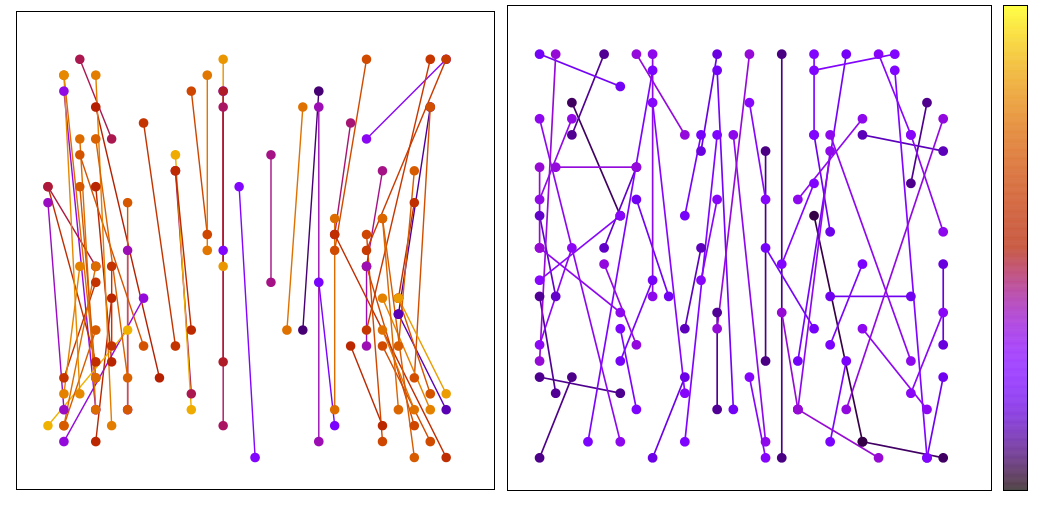
\includegraphics[width=\imsize]
{correlacion-orb}
\caption[Comparación tests binarios con y sin aprendizaje ORB.]
{Izquierda: conjunto de tests binarios obtenidos sin aprendizaje (utilizando la orientación y el enfoque de BRIEF para seleccionar los tests). Derecha: conjunto de tests binarios obtenidos por medio del algoritmo de aprendizaje. El color violeta indica poco correlación, mientras que el color naranja representa alta correlación. Se puede observar que los tests aprendidos tienen una mejor distribución y están menos correlacionados. Imagen original : \cite{RubleeRKB11}.}
\label{fig:correlacion-orb}
\end{figure}

Para la construcción de cada descriptor, se utiliza la orientación obtenida en la fase de detección como sigue :
\begin{enumerate}

\item Se construye la matriz \textit{S} con las coordenadas de los pares de puntos para tests obtenidos con el enfoque de aprendizaje.

\begin{equation}
S =
\left(
\begin{array}{ccc}
\textbf{x}_{1},& ..., &\textbf{x}_{n} \\
\textbf{y}_{1},& ..., &\textbf{y}_{n} \\
\end{array}
\right)
\end{equation}

\item A partir de la orientación $\theta$ del \textit{patch}, se construye la correspondiente matriz de rotación $R_{\theta}$ y se obtiene la versión rotada $ S_{\theta} $ de \textit{S}.
\begin{equation}
S_{\theta} = R_{\theta}S
\end{equation}
\item Por último, se utiliza el operador de BRIEF $f_{n}(\textbf{p})$ sobre los tests rotados, obteniendo el operador de rBRIEF.
\begin{equation}
g_{n}(\textbf{p}, \theta) := f_{n}(\textbf{p})|(\textbf{x}_{i}, \textbf{y}_{i}) \in S_{\theta}
\end{equation}

\end{enumerate}

En la implementación, el algoritmo de aprendizaje se lleva a cabo en un proceso \textit{offline}. Además, se discretizan los ángulos en incrementos de $2\pi/30$ (12 grados) y se construye una \textit{lookup-table} de patrones punto-ángulo precalculados.

\section{Correspondencia de características}

\subsection{Correspondencia de características 2D}
En la sección \ref{sec:features}, se describe el concepto de detección y representación (construyendo un descriptor) de características visuales. El descriptor es un vector de tamaño fijo, que permite establecer correspondencias entre características observadas en distintas imágenes. \\
Dado conjuntos de descriptores origen y destino, el procedimiento para establecer correspondencias consiste en hallar, para cada elemento del conjunto de origen, el elemento más próximo en el conjunto de destino.

% AGREGAR FIGURA QUE MUESTRE UN MATCHING.

El concepto de distancia suele definirse en función de la naturaleza del descriptor :
\begin{itemize}

\item Cuando los componentes del descriptor son reales (por ejemplo SURF, SIFT) usualmente se utiliza la norma euclídea.

\item Cuando las componentes son binarios (por ejemplo ORB, BRIEF) se utiliza (debido a su eficiencia) la distancia de Hamming\footnote{Dados de vectores binarios, la distancia de Hamming se define como la cantidad de bits que difieren los vectores.}.

\end{itemize}

Para evitar correspondencias incorrectas, se utiliza un umbral que descarta pares de características muy distantes (en el espacio de dimensiones del descriptor). \\

El problema del emparejamiento de características tiene un alto costo computacional cuando se comparan grandes conjuntos de datos y/o cuando es elevada la dimensión de los descriptores. Para abordar este inconveniente, se hace uso de estructuras y algoritmos que resuelven el problema de encontrar el vecino más cercano (\textit{nearest neighbor search}) de forma muy eficiente. Según el tipo de distancia empleada, se utilizan diferentes enfoques. Para el caso de la norma euclídea, las búsquedas de proximidad se apoyan en árboles k-dimensionales (\textit{kd-tree})\cite{wiki-kdtree}, que siguen un enfoque de particionado del espacio de búsqueda\cite{wiki-particionado-espacio}. Por otro lado, cuando se emplea la distancia de Hamming, el enfoque utilizado es \textit{Locality-sensitive hashing (LSH)}\cite{wiki-lsh}, que se basa en una reducción probabilística del espacio.

\subsection{Extracción de puntos 3D y definición de correspondencias 3D}

En última instancia, para cada punto 2D en una correspondencia obtenida en el apartado anterior, se le asocia un punto 3D. Esta simple asociación es posible debido a que la nube de puntos RGB-D capturada por la Kinect es una composición de los frames RGB y de profundidad que este sensor provee, es decir, un frame RGB-D con la misma organización espacial que las imágenes 2D. \\
En la sección \ref{sec:consideraciones-kinect} se explica que debido a la disposición interna de los sensores IR de la cámara Kinect pueden existir áreas de la escena sin mediciones de profundidad (pero posiblemente con valores RGB). Teniendo en cuenta lo anterior, se descartan las correspondencias que no pueden ser asociadas a pares de puntos 3D válidos.

\section{Aproximación y refinamiento de la transformación rígida}
\label{sec:transformacion-rigida}

Encontrar la transformación rígida óptima entre 2 conjuntos de puntos 3D es una tarea fundamental en la reconstrucción de mapas 3D. El problema se ilustra en la figura \ref{fig:esquema-encontrar-transformacion} para el caso más simple de 3 correspondencias (mínimo requerido). El objetivo es encontrar la transformación \textbf{T} que mejor alinea el conjunto \textbf{A} con el conjunto \textbf{B}, en otras palabras, se desea computar la traslación \textbf{t} y rotación \textbf{R} que minimiza el error cuadrático medio (MSE) dado por:
\begin{equation}
\label{ec:mse-rigid-transform}
error = \sum_{i = 1}^{N} \norm{\textbf{T} P_{A}^{i} - P_{B}^{i}} = \sum_{i = 1}^{N} \norm{\textbf{R} P_{A}^{i} + \textbf{t} - P_{B}^{i}}
\end{equation}
donde \textit{$P_{A}^{i}$}, \textit{$P_{B}^{i}$} son puntos 3D en \textbf{A} y \textbf{B} respectivamente (en correspondencia dada por el índice i).

\begin{figure}[ht]
\centering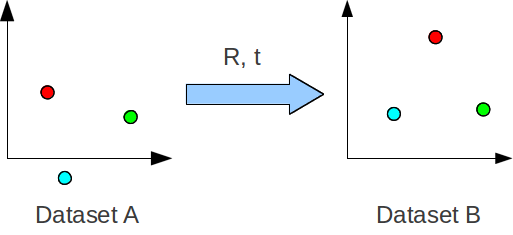
\includegraphics[width=\imsize]
{esquema-encontrar-transformacion}
\caption[Cómputo de la transformación rígida a partir de 3 correspondencias]
{Cómputo de la transformación rígida a partir de 3 correspondencias}
\label{fig:esquema-encontrar-transformacion}
\end{figure}

En esta sección, se presentan 2 algoritmos que en conjunto abordan el problema de encontrar la transformación rígida. En primer lugar, se presenta un método directo para estimar la transformación a partir de un conjunto de correspondencias 3D y a continuación, se explica un algoritmo iterativo que permite refinar la transformación a partir de una estimación inicial.

\subsection{Estimación de la transformación rígida utilizando SVD}
El algoritmo directo presentado en este apartado requiere al menos 3 correspondencias de puntos 3D para poder aplicarse y asume que estas son correctas.

Consideremos $P_{A}^{i}, P_{B}^{i}$ como las correspondencias de las nubes de puntos \textbf{A}, \textbf{B} (con \textit{N} elementos).
El algoritmo para aproximar la transformación rígida se divide en los siguientes pasos:
\begin{enumerate}

\item Encontrar los centroides para ambos conjuntos.
\begin{equation}
centroid_{A} = \frac{1}{N} \sum_{i = 1}^{N} P_{A}^{i}
\end{equation}
\begin{equation}
centroid_{B} = \frac{1}{N} \sum_{i = 1}^{N} P_{B}^{i}
\end{equation}

\item Centrar ambos conjuntos, de forma tal que ambos centroides están en el origen de coordenadas.
\begin{equation}
CP_{A}^{i} = P_{A}^{i} - centroid_{A}
\end{equation}
\begin{equation}
CP_{B}^{i} = P_{B}^{i} - centroid_{B}
\end{equation}
donde $CP_{A}^{i}, CP_{B}^{i}$ (para $i=1,..,N$) denotan los respectivos conjuntos centrados en el origen.

\item Definir la matriz de covarianza
\begin{equation}
H = \sum_{i} CP_{A}^{i} (CP_{B}^{i})^{T}.
\end{equation}

\item Encontrar la factorización por descomposición en valores singulares (SVD, por sus siglas en inglés)\cite{wiki-svd} de H, definida por
\begin{equation}
H = U \Sigma V^{T}
\end{equation}
y estimar la matriz de rotación \textbf{R} como sigue:
\begin{equation}
\textbf{R} = V U^{T}
\end{equation}

\item Finalmente, la traslación \textbf{t} se calcula como:
\begin{equation}
\textbf{t} = centroid_{B} - \textbf{R} centroid_{A}
\end{equation}

\end{enumerate}

Este método es uno de los más simple para obtener la rotación y traslación entre dos nubes de puntos, pero tiene el inconveniente que supone que una de ellas es una versión trasladada y rotada de la otra. Por lo general, no es recomendable hacer esta suposición debido a que las correspondencias pueden ser incorrectas o estar afectadas por ruido. En la sección \ref{sec:ransac}, se explica el algoritmo RANSAC, que permite encontrar un conjunto consistente de correspondencias para ser utilizadas con el procedimiento descripto en esta sección.

\subsection{Refinamiento de la transformación rígida utilizando ICP}

El algoritmo Iterative Closest Point (ICP) \cite{Besl92} surgió a principios de los noventa como solución al problema de scan-matching, es decir, encontrar la mejor transformación que minimiza la distancia entre dos nubes de puntos relevadas con sensores de rango. La principal desventaja del algoritmo original es que asume superposición total de las nubes de puntos a alinear y que los puntos no tienen error. Desde entonces se han propuesto algunas variantes de ICP enfocadas en mejorar su precisión y eficiencia.\\
ICP toma como parámetros de entradas dos nubes de puntos $\textbf{A} = \{a_{i}\}, \textbf{B} = \{b_{i}\}$ y una transformación inicial $\textbf{T}_{0}$ que acerca la nube de puntos \textbf{A} con \textbf{B}, y devuelve la transformación \textbf{T} que mejor alinea ambas nubes de puntos, resolviendo un problema de minimización. Debido a que ICP busca un mínimo local, puede ocurrir que no converga a una solución óptima si $\textbf{T}_{0}$ no es una aproximación suficientemente buena. \\

A continuación, se presenta la versión estándar de ICP en pseudocódigo :
\begin{algorithm}
\begin{algorithmic}

\STATE $\textbf{T} \leftarrow \textbf{T}_{0}$
\WHILE {not converged}
\FOR{$i \leftarrow 1 to N$}
\STATE $m_{i} \leftarrow FindClosestPointInB(\textbf{T} a_{i})$
\IF{ $(\norm{ T a_{i} - m_{i} } )^{2} \geq d_{max}$ }
\STATE $w_{i} \leftarrow 1$
\ELSE
\STATE $w_{i} \leftarrow 0$
\ENDIF
\ENDFOR
\STATE $ \textbf{T} \leftarrow \underset{\textbf{T}}{\arg\min}  \underset{i}{\sum} w_{i} (\norm{ \textbf{T}a_{i} - m_{i} })^{2} $
\ENDWHILE

\end{algorithmic}
\caption{Pseudocódigo ICP estándar}
\label{icp-pseudocodigo}
\end{algorithm}

Conceptualmente cada iteración ICP se divide en las siguiente etapas :
\begin{enumerate}

\item Determinar las correspondencias entre los conjuntos \textbf{A} y \textbf{B}. Para esto se transforma cada punto en \textbf{A} (con la mejor transformación hasta esa iteración) y se busca el vecino más cercano en \textbf{B} (se utilizan \textit{kd-trees}\cite{wiki-kdtree} para acelerar la búsqueda).

\item Eliminar \textit{outliers}. Si la distancia de $m_{i}$ a $\textbf{T}a_{i}$ es mayor a cierto umbral $d_{max}$, la correspondencia se descarta. Esto permite aceptar nubes de puntos que no estén completamente sobrelapadas y disminuye el error en el paso de minimización.

\item Estimar la transformación rígida que minimiza las distancias entre las correspondencias (minimiza la ecuación \ref{ec:mse-rigid-transform}).

\end{enumerate}

Este proceso se repite iterativamente hasta que se cumpla alguna de las condiciones de convergencia.
Los criterios de convergencia más comunes son :
\begin{itemize}
\item Alcanzar límite de iteraciones.

\item MSE definido en la ecuación \ref{ec:mse-rigid-transform} (para las nubes de puntos alineadas) cae por debajo de cierto umbral.

\item Diferencia entre las transformaciones obtenidas en iteraciones consecutivas por debajo de cierto umbral.
\end{itemize}

\section{RANdom SAmple Consensus (RANSAC)}
\label{sec:ransac}
RANSAC \cite{Fischler81} es un método iterativo para estimar los parámetros de un modelo matemático a partir de un conjunto de observaciones, que puede contener valores espurios (obtenidos por mediciones erróneas o hipótesis incorrectas). RANSAC establece dos subconjuntos, uno con los datos que pueden ser explicado por el modelo (\textit{inliers}), y otro con los datos que no ajustados por el modelo (\textit{outliers}). También asume que existe un procedimiento, tal que a partir de un conjunto pequeño de \textit{inliers}, se puede estimar los parámetros del modelo que mejor ajusta al conjunto total de \textit{inliers}. \\
Generalmente, utilizando un enfoque de cuadrados mínimos, se encuentra una instancia de los parámetros que mejor satisface el conjunto completo de los datos, pero que probablemente no es la solución óptima, debido a la presencia de ruido. RANSAC propone encontrar parámetros que son válidos para la mayoría de los puntos (un consenso), descartando los puntos con ruido. En la figura \ref{fig:ransac-line2d} se muestra la aplicación de RANSAC para estimar una recta 2D.

\begin{figure}[ht]
\centering
\begin{minipage}[h]{.45\textwidth}
\begin{center}
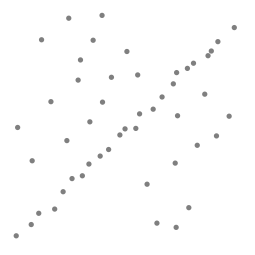
\includegraphics[width=\imsizeS]{ransac-line1}
\end{center}
\end{minipage}
\hfill
\begin{minipage}[h]{.45\textwidth}
\begin{center}
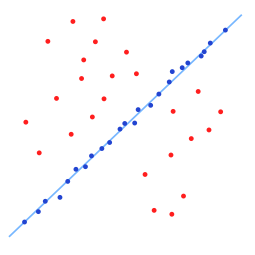
\includegraphics[width=\imsizeS]{ransac-line2}
\end{center}
\end{minipage}
\hfill
\caption[RANSAC para estimar una recta 2D]
{Izquierda: conjunto de datos con muchos \textit{outliers} para los que se desea ajustar una recta. Derecha: línea ajustada por RANSAC. Se observa que los valores espurios no afectan el resultado. Imágenes originales extraídas de Wikipedia bajo licencia Creative Commons.}
\label{fig:ransac-line2d}
\end{figure}

Los parámetros de entrada para RANSAC son :
\begin{itemize}

\item El conjunto total de \textsl{M} observaciones.
\item Un modelo que puede estimarse usando \textsl{N} observaciones.
\item La cantidad de iteraciones \textsl{L} que debe ejecutarse.
\item Un valor de tolerancia \textsl{t} para determinar cuando una observación se ajusta al modelo.
\item La cantidad mínima \textsl{D} de observaciones para considerar que un modelo ajusta bien.

\end{itemize}

El algoritmo estándar RANSAC se describe como :
\begin{enumerate}

\item Seleccionar un conjunto \textbf{S} con \textsl{N} observaciones aleatorias (hipotéticos \textit{inliers}) a partir del conjunto total.

\item Estimar el vector de parámetros \textbf{x} que describen el modelo, a partir de \textbf{S}.

\item Encontrar el conjunto \textbf{C} (consenso) de observaciones a partir del conjunto total, que ajustan al modelo descrito por \textbf{x} con una tolerancia \textsl{t}.

\item Si el modelo estimado es razonablemente bueno ($\abs{\textbf{C}} > \textsl{D} $), se estima un nuevo modelo a partir de \textbf{C} y se mantiene la estimación más precisa hasta el momento.

\item Se repite los pasos 1 a 4 hasta alcanzar \textsl{L} iteraciones.
\end{enumerate}

\subsection{Eliminación de correspondencias 3D erróneas con RANSAC}

En el presente trabajo, se aplica RANSAC en la estimación de la transformación rígida, con el objetivo de aumentar su robustez ante correspondencias erróneas. En este caso, el modelo que se trata de estimar es la matriz \textbf{T} de $4\times4$, que mejor ajusta la traslación y rotación dada por los pares de puntos 3D en correspondencia. Como se menciona en \ref{sec:transformacion-rigida}, se necesitan al menos 3 correspondencias para estimar los parametros de \textbf{T}. Tras estimar el modelo en cada iteración, se consideran \textit{inliers} aquellos pares de puntos 3D $\textbf{x}_{i} \leftrightarrow \textbf{x'}_{i}$ que cumplen que la distancia de $\textbf{x'}_{i}$ a $ \textbf{T}\textbf{x}_{i}$ es menor que un determinado umbral. En la figura \ref{fig:ransac-rigid-transform} se ilustra el criterio para determinar \textit{inliers} y \textit{outliers}.

\begin{figure}[ht]
\centering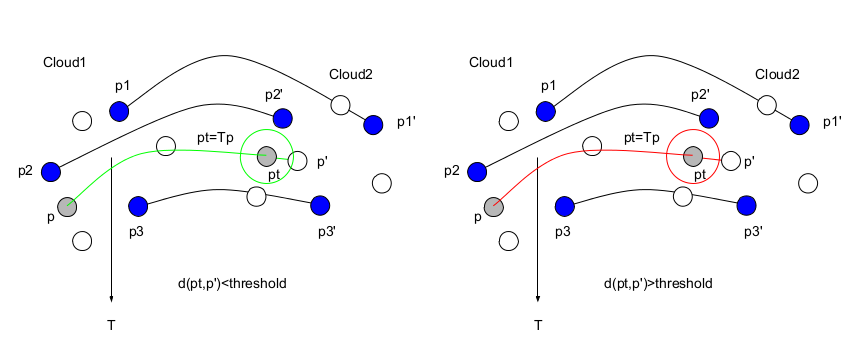
\includegraphics[width=\imsizeL]
{ransac-rigid-transform}
\caption[Eliminación de correspondencias 3D erróneas]
{Eliminación de outliers 3D con la transformación rígida \textbf{T} basándose en la distancia de \textbf{p'} a la correspondencia transformada $\textbf{p}_{t} = \textbf{T}\textbf{p}$. Izquierda: la distancia de la correspondencia \textbf{p'} de \textbf{p} al punto transformado $\textbf{p}_{t}$ es menor de un cierto umbral, por lo que se considera \textit{inlier}. Derecha: la distancia de \textbf{p} al punto transformado $\textbf{p}_{t}$ es mayor que un cierto umbral, por lo que se considera \textit{outlier}.}
\label{fig:ransac-rigid-transform}
\end{figure}

\section{El problema de la acumulacion de error y la solución utilizando SLAM}
\label{sec:acumulacion-del-error-slam}

En las secciones previas, se describe cómo estimar la pose de la cámara mediante un método de alineación de nubes de puntos. Esta alineación puede ser imprecisa, debido a la presencia de ruido en el sensor o correspondencias incorrectas. Para llevar a cabo la registración de imágenes que permita construir un mapa 3D es necesario determinar la pose global de la cámara para cada imagen. La desventaja de utilizar sólo un enfoque de odometría visual radica en que la estimación de la pose global se obtiene componiendo las transformaciones (o poses) relativas previas, lo que conduce a una acumulación del error. Con el paso del tiempo, el error acumulado provoca que el mapa deje de ser útil. \\
Para enfrentar este problema, se presenta una técnica de optimización global, conocida como \textit{Simultaneous Localization And Mapping (SLAM)} que permite estimar una trayectoria globalmente consistente, a partir de mediciones que contienen error, realizando varias observaciones de un mismo lugar. De esta forma, se evita la acumulación del error en las poses y permite generar mapas globalmente consistentes. En la figura \ref{fig:maps-noisy-slam}, se puede observar un mapa afectado por la acumulacion de error (izquierda) y el mapa resultante de aplicar SLAM (derecha). \\

\begin{figure}[ht]
\centering
\begin{minipage}[h]{.45\textwidth}
\begin{center}
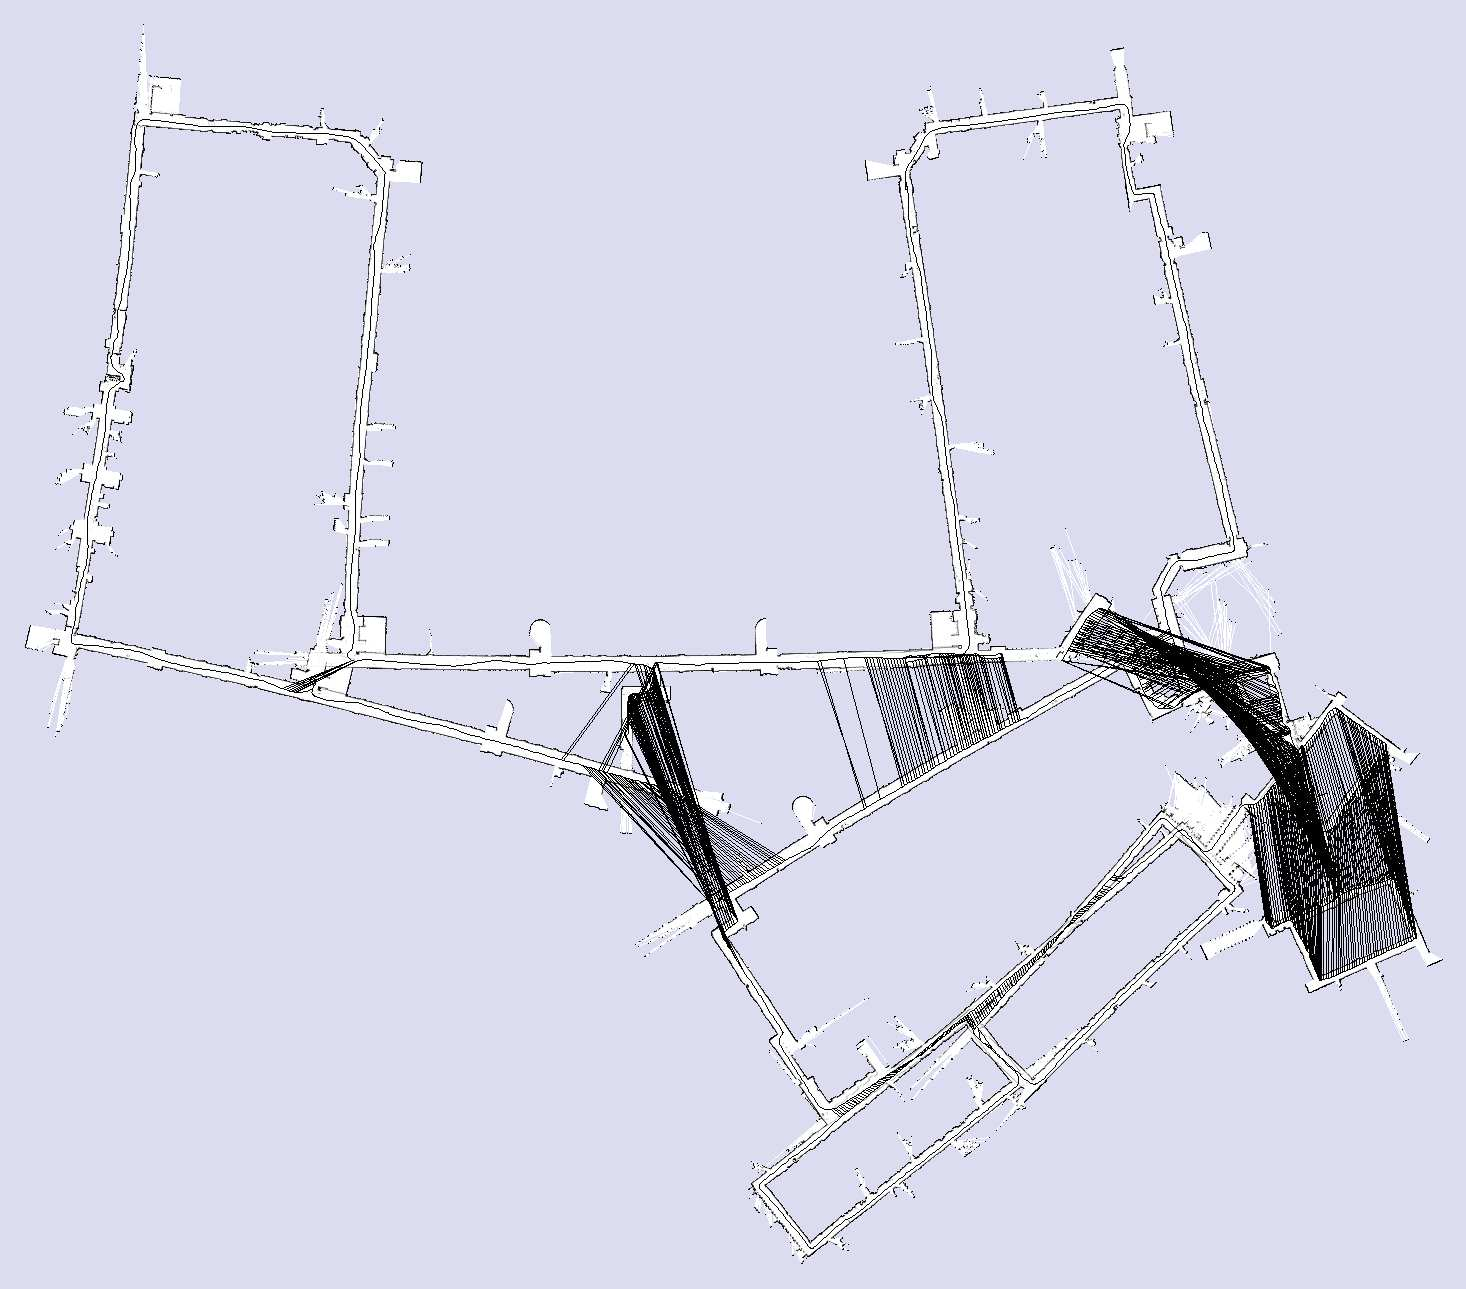
\includegraphics[width=\imsizeS]{noisy-map}
\end{center}
\end{minipage}
\hfill
\begin{minipage}[h]{.45\textwidth}
\begin{center}
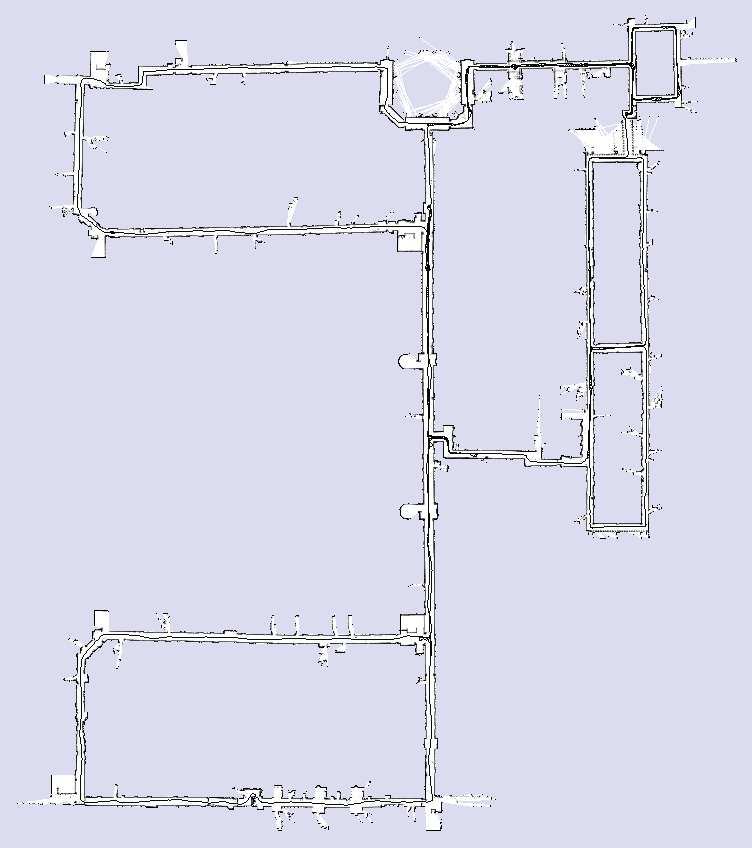
\includegraphics[width=0.95\textwidth]{slam-map}
\end{center}
\end{minipage}
\hfill
\caption[Efecto de la acumulacion del error y optimización con SLAM sobre un mapa]
{Izquierda: mapa inconsistente afectado por la acumulacion del error. Derecha: Mapa refinado por SLAM.Imágeness originales : \cite{GrisettiKSB10}.}
\label{fig:maps-noisy-slam}
\end{figure}

\subsection{Simultaneous Localization And Mapping (SLAM)}

SLAM plantea la problemática de que un robot (de forma general, un sistema sensorial) pueda construir un mapa incrementalmente del entorno y al mismo tiempo determinar su ubicación dentro del mapa, sin conocimiento a priori de su ubicación inicial. La solución al problema SLAM ha sido objeto de estudio de la comunidad de robótica móvil durante los últimos 20 años. SLAM ha sido planteado y resuelto teóricamente de diferentes formas, y aplicado en áreas diversas de la robótica, tales como robots en interiores, exteriores, subacuáticos, incluso sistemas aéreos. La presencia de ruido en el sistema sensorial, los inevitables errores, aproximaciones efectuadas en los modelos empleados y la complejidad creciente al procesar mayor cantidad de información, han sido inconvenientes en la aplicación práctica de soluciones SLAM, por lo que sigue siendo área de investigación. Debido a la presencia del error en las mediciones del sensor, las soluciones más exitosas se han basado en herramientas probabilísticas.

\subsubsection{Formulación probabilística de SLAM}

La formulación clásica de SLAM asume que el sensor se desplaza en un entorno desconocido siguiendo la trayectoria $\textbf{x}_{1:T} = \{\textbf{x}_{1}, ..., \textbf{x}_{T}\}$ en intervalos discretos de tiempo 1 a \textsl{T}. Durante su recorrido, el sensor releva medidas de odometría $\textbf{u}_{1:T} = \{\textbf{u}_{1}, ..., \textbf{u}_{T}\}$ y toma conjuntos de observaciones (puntos de interés) $\textbf{z}_{1:T} = \{\textbf{z}_{1}, ..., \textbf{z}_{T}\}$. Resolver SLAM consiste en estimar la probabilidad a posteriori de la trayectoria del $\textbf{z}_{1:T}$ y el mapa \textbf{m} del entorno dadas las mediciones y la posición inicial $\textbf{x}_{0}$:
\begin{equation}
p(\textbf{x}_{1:T}, \textbf{m} | \textbf{z}_{1:T}, \textbf{u}_{1:T}, \textbf{x}_{0}).
\end{equation}
Las poses $\textbf{x}_{1:T}$ y las mediciones de odometría $\textbf{u}_{1:T}$ suelen representarse como transformaciones 2D o 3D, mientras que las formas más comunes para representar el mapa son puntos de interés distribuidos en el espacio, \textit{occupancy grids} e incluso el conjunto completo medido por el sensor. \\
En la práctica, resolver el problema SLAM requiere:
\begin{itemize}

\item Un modelo para actualizar la posición, que representa la probabilidad $p(\textbf{x}_{t} | \textbf{x}_{t-1}, \textbf{u}_{t})$ de estar en la posición $\textbf{x}_{t}$ en el instante \textsl{t}, dado que en \textsl{t-1} estaba en $\textbf{x}_{t-1}$ y se midió la odometría $\textbf{u}_{t}$.

\item Un modelo de observación, que representa la probabilidad $p(\textbf{z}_{t} | \textbf{x}_{t}, \textbf{m})$ de hacer una observación $\textbf{z}_{t}$ dado que el sensor se encuentra en la posición $\textbf{x}_{t}$ en el mapa \textbf{m}.

\end{itemize}

\begin{figure}[ht]
\centering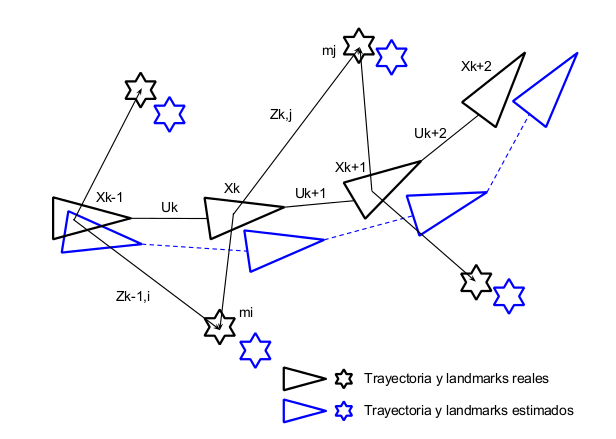
\includegraphics[width=\imsize]
{slam-esquema}
\caption[Formulación SLAM]
{El problema esencial de SLAM. Se requiere una estimación simultánea tanto de la localización del sensor como de los landmarks. Las localizaciones reales no se pueden conocer ni medir directamente debido a las limitaciones del sensor. Las observaciones se toman entre el sensor real y las localizaciones de los \textit{landmarks}.}
\label{fig:slam-esquema}
\end{figure}

\subsubsection{Solución \textit{GraphSLAM}}

La literatura presenta diferentes técnicas para resolver este problema. Tradicionalmente, se han utilizado soluciones basadas en Filtros de Kalman extendido\cite{wiki-ekf} y filtros de partículas\cite{wiki-filtro-de-particulas}. Una alternativa más reciente es la denominada \textit{GraphSLAM}. En la representación \textit{GraphSLAM}, las poses del sensor se representan como nodos en un grafo, mientras que las restricciones espaciales entre las poses, obtenidas a partir de las observaciones y la odometría, se modelan como aristas. Una vez que el grafo está construido, se trata de buscar la configuración de las poses del sensor que mejor satisfacen las restricciones. En la figura \ref{fig:graphslam-frontend-backend} se ilustra un sistema típico \textit{GraphSLAM}. Conceptualmente, el sistema se divide en 2 tareas:

\begin{enumerate}

\item Construcción del grafo, conocido en la literatura como \textit{front-end}.

\item Optimización del grafo, también conocido como \textit{back-end}.

\end{enumerate}

\begin{figure}[ht]
\centering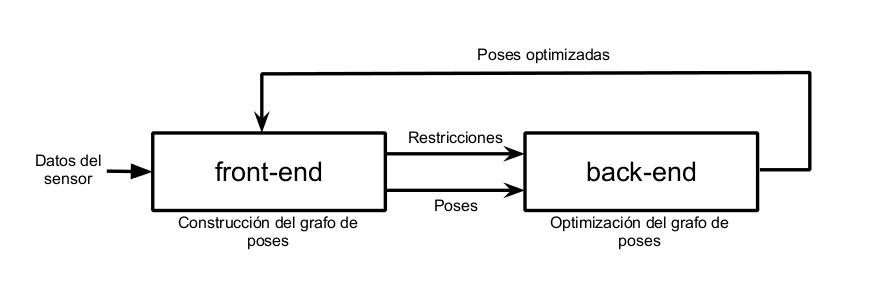
\includegraphics[width=\imsizeL]
{graphslam-frontend-backend}
\caption[Sistema GraphSLAM \textit{front-end} y \textit{back-end}]
{Sistema típico de \textit{GraphSLAM}. El \textit{front-end} y \textit{back-end} del algoritmo se ejecutan de forma intercalada. \textit{El front-end} se encarga de estimar las poses del sensor a lo largo de su trayectoria y de estimar una serie de restricciones espaciales entre las poses con las que construir el grafo. El \textit{back-end} se encarga de encontrar la configuración de parametros que mejor satisface las restricciones impuestas por las aristas del grafo.}
\label{fig:graphslam-frontend-backend}
\end{figure}

\paragraph{El grafo de poses y restricciones espaciales}

La técnica de \textit{GraphSLAM} construye un grafo que representa la topología del entorno por donde se mueve el sensor. En la figura \ref{fig:grafo-graphslam} se observa la estructura del grafo, donde cada nodo $\textbf{x}_{t}$ posee la posición del sensor en el instante \textsl{t} y cada arista $\textbf{e}_{ij}$ contiene las restricciones espaciales entre los nodos \textsl{i, j}. Las poses consecutivas modelan mediciones de odometría, mientras que aristas entre poses no consecutivas representan restricciones espaciales que se agregan a partir de múltiples observaciones de la misma zona.\\
Detectar zonas por donde ya se ha pasado anteriormente, se conoce en la literatura como \textit{detección de bucles}, debido al hecho a que da lugar a trayectorias cerradas. También se utiliza el término \textit{cierre de bucles}, para indicar la acción de detectar una zona ya visitada y utilizar esta información para optimizar el grafo.

\begin{figure}[ht]
\centering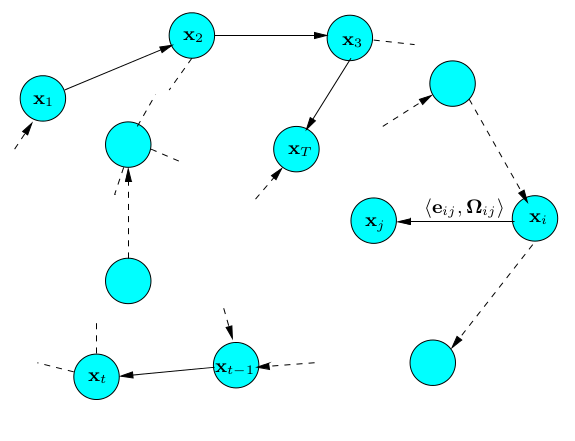
\includegraphics[width=\imsize]
{grafo-graphslam}
\caption[Representación de SLAM con un grafo de poses]
{Cada nodo representa una pose del sensor. Las aristas representan restricciones espaciales entre los nodos.}
\label{fig:grafo-graphslam}
\end{figure}

\paragraph{\textit{\textsl{Front-end}} : detección de bucles y construcción del grafo de poses}
\label{sec:slam-frontend}

En este trabajo, se sigue un enfoque de detección de bucles similar al presentado en \cite{henry2010rgb}, que si bien se caracteriza por ser sencillo, sirve para construir grafos (pequeños) que se ajustan a los requerimientos para mapear una superficie en laboratorio. \\
El proceso de construcción del grafo utiliza la técnica de alineación de frames presentada en la sección \ref{sec:descripcion-general-registracion} en 2 instancias diferentes, en primer lugar para calcular la odometría entre cada desplazamiento y de forma seguida, para detectar posibles bucles. En ambas etapas se utiliza la cantidad de correspondencias consistentes (habiendo aplicado RANSAC \ref{sec:ransac}) para determinar la calidad de la transformación. \\
Para obtener la odometría (desplazamiento del sensor) desde $\textbf{x}_{t-1}$ a $\textbf{x}_{t}$, se aplica la alineación entre los frames capturados en dichas posiciones, resultando en la transformación relativa $\textbf{u}_{t}$. Si la cantidad de correspondencias consistentes es superior a un umbral $n_{u}$, se considera que la transición pudo ser medida exitosamente, lo que permite extender el grafo con $\textbf{x}_{t} = \textbf{u}_{t} \textbf{x}_{t-1}$ y la restricción espacial determinada por $\textbf{u}_{t}$. Si se fracasa en estimar la odometría, el frame se descarta y el grafo se mantiene inalterado. \\
Para llevar a cabo la detección de bucles, se alinea el frame actual con los frames previos (asociados a poses en el grafo). Si el número de correspondencias consistentes es superior a un umbral $n_{e}$, se considera que se ha vuelto a pasar por un lugar visitado anteriormente. En tal caso, se añade una arista (restricción espacial) entre dicha pose y la actual. Si no se alcanza $n_{e}$, se concluye que los frames no visualizan la misma zona. En la implementación, se utiliza la información de la poses (posición y orientación) para determinar frames próximos al actual y evitar el proceso de alineación entre frames muy alejados, que probablemente no puedan aportar restricciones espaciales nuevas. \\
En base a los experimentos realizados en el Laboratorio de Hidráulica en el marco de este trabajo, se determinó que se requieren alrededor $n_{e} = 25$ correspondencias para determinar si una escena es revisitada. Para estimar la odometría, se seteo $n_{u} = 45$ teniendo en cuenta que entre frames consecutivos la transformación debe ser precisa y el porcentaje de área sobrelapada debería ser cercano al 50\%. \\
En la implementación es posible limitar la cantidad de aristas que se agregan en la etapa detección de bucles para reducir el costo computacional de esta etapa.

\paragraph{\textit{Back-end}: Optimización del grafo de poses}

Considere $\textbf{x} = (\textbf{x}_{1}, ..., \textbf{x}_{T})^{T}$ un vector donde cada componente $\textbf{x}_{i}$ contiene el nodo \textsl{i}. Además, para cada restricción espacial, entre nodos \textsl{i, j}, se les puede asociar una medición $\textbf{z}_{ij}$ con distribución Normal de media $\hat{\textbf{z}_{ij}}$ y matrix de información $\Omega_{ij}$ (inversa de la matriz de covarianza $\Sigma_{ij}$). \\
Utilizando el criterio máxima de verosimilitud, tenemos que la función de verosimilitud o de probabilidad conjunta \cite{wiki-mle} sobre todas las mediciones $\textbf{z}_{ij}$ se define como :

\begin{equation}
\prod{\textbf{z}_{ij}}
\end{equation}

y el logaritmo de la función de verosimilitud esta dado por :

\begin{equation}
\ln \prod{\textbf{z}_{ij}} = \sum{\ln \textbf{z}_{ij}} = \sum{\textit{\textbf{l}}_{ij}}
\end{equation}

donde $\textit{\textbf{l}}_{ij}$ es el logaritmo de la distribución $\textbf{z}_{ij}$

\begin{equation}
\textit{\textbf{l}}_{ij} \propto (\textbf{z}_{ij}-\hat{\textbf{z}}_{ij}(\textbf{x}_{i},\textbf{x}_{j}))^{T}\Omega_{ij}(\textbf{z}_{ij}-\hat{\textbf{z}}_{ij}(\textbf{x}_{i},\textbf{x}_{j}))
\end{equation}

Considérese \textbf{C} el conjunto de pares de índices para los que existe una restricción u observación \textbf{z}. Encontrar el estimador de máxima verosimilitud (MLE) consiste en encontrar la configuración de los nodos $\textbf{x}^{*}$ que minimiza la función \textit{L(\textbf{x})} de todas las observaciones, es decir,
\begin{equation}
\textbf{x}^{*} = \underset{\textbf{x}}{\arg\min} L(x) = \underset{\textbf{x}}{\arg\min} \sum_{<i,j>\in \mathcal{\textbf{C}}}\textbf{e}_{ij}^{T}\Omega_{ij}\textbf{e}_{ij}
\end{equation}
con $\textbf{e}_{ij}(\textbf{x}_{i},\textbf{x}_{j})=\textbf{z}_{ij}-\hat{\textbf{z}}_{ij}(\textbf{x}_{i},\textbf{x}_{j})$ el error entre la medición y su valor esperado.
Cabe notar que se requiere minimizar la suma, dado que los términos individuales $\textit{\textbf{l}}_{ij}$ son técnicamente la negación del logaritmo de la distribución $\textbf{z}_{ij}$.

\begin{figure}[ht]
\centering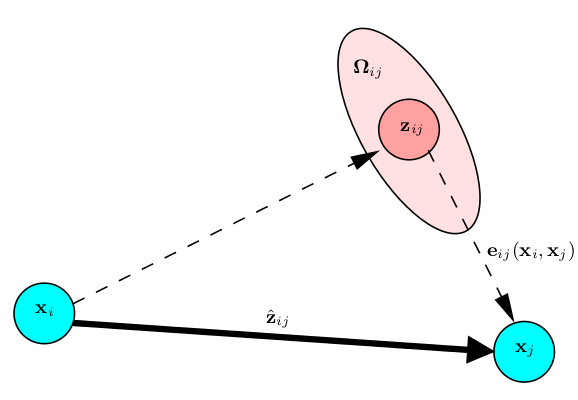
\includegraphics[width=\imsize]
{arista-graphslam}
\caption[Arista del grafo de poses en \textit{GraphSLAM}]
{Aspecto de una arista que conecta los vértices $\textbf{x}_{i}, \textbf{x}_{j}$. Esta arista se origina a partir de la medición $\textbf{z}_{ij}$. Dadas las posiciones de dos nodos, es posible computar la medición esperada $\hat{\textbf{z}}_{ij}$ que representa $\textbf{x}_{j}$ visto desde $\textbf{x}_{i}$. El error $\textbf{e}_{ij}(\textbf{x}_{i},\textbf{x}_{j})$ depende del desplazamiento entre la medida real y la esperada. Una arista se caracteriza completamente por su función de error $\textbf{e}_{ij}(\textbf{x}_{i},\textbf{x}_{j})$ y por la matriz de información $\Omega_{ij}$ de la medida que tiene en cuenta su incertidumbre.}
\label{fig:arista-graphslam}
\end{figure}

En este trabajo, el problema de minimización se resuelve por medio del enfoque aplicado en \cite{lingemannefficient}, basado en la propuesta original de \textit{GraphSLAM} presentada por Lu y Milios\cite{Lu97globallyconsistent} (1997).